\documentclass{bioinfo}

\copyrightyear{2014}

\pubyear{2014}

\begin{document}

\firstpage{1}

\title{Chemistry Aware Model Builder (camb): An R package for bioactivity and property modeling of small molecules and proteins}
\author[Murrell \& Cortes-Ciriano \it{et~al}]{Daniel S. Murrell\,$^{1}$\footnote{Equal contributors} , Isidro Cortes-Ciriano\,$^{2,*}$, Gerard J.P. van Westen\,$^{3}$, Th\'er\`ese E. Malliavin\,$^{2,}$\footnote{to whom correspondence should be addressed} , Andreas Bender$^{1,}$\dag}
\address{$^{1}$Unilever Centre for Molecular Science Informatics, Department of Chemistry, University of Cambridge, Cambridge, United Kingdom.\\
$^{2}$Unite de Bioinformatique Structurale, Institut Pasteur and CNRS UMR 3825, Structural Biology and Chemistry Department, 25\-28, rue Dr. Roux, 75 724 Paris, France.\\
$^{3}$European Molecular Biology Laboratory European Bioinformatics Institute Wellcome Trust Genome Campus, Hinxton, United Kingdom.}

\history{Received on XXXXX; revised on XXXXX; accepted on XXXXX}
\editor{Associate Editor: XXXXXXX}
\maketitle

\begin{abstract}
\section{Summary:}
{\it camb} is an R package for the generation of quantitative predictive models
for medicinal chemistry (QSAR, QSPR, QSAM, proteochemometrics and chemogenomics). 
Its functionalities enable the standardization and representation of chemical structures.
Moreover, 905 2-dimensional descriptors, and 14 types of fingerprints (among which circular Morgan 
fingerprints) can be computed. 
Similarly, {\it camb} allows the calculation of 8 types of amino acid descriptors and 13 different whole protein sequence descriptors.
Finally, statistical preprocessing of descriptors and the generation of machine learning models (single models or ensemble modeling) through
the R package caret is also supported.
Results can be visualized through high-quality and customizable plots based on ggplot2. 
Overall, {\it camb} constitutes a useful tool for the generation of predictive models 
for both amateur and advanced users.\\
\section{Availability:} {\it camb} is written in R, C, python and Java and is freely available
at https://github.com/cambDI/camb.
Two tutorials are also included.\\
\section{Contact:} dsmurrell@gmail.com and isidrolauscher@gmail.com
%\href{terez@pasteur.fr, ab454@cam.ac.uk}
\end{abstract}


\section{Introduction}

The advent of high-throughtput technologies over the last two decades 
has led to a vast increase of compounds bioactivity
and genomic databases \citep{bender_databases}.
This large-scale amount of chemical and biological information 
has been exploited by emergent fields in drug discovery 
such as chemogenomics or proteochemometrics (PCM) \citep{review_pcm,cortesReview}.
%In this line, a plethora of studies have proved the usefulness of {\it in silico}
%approaches for drug repurposing \citep{iorio}, target prediction \citep{cortes,alexios},
%receptor deorphanization \citep{bredel}, and the discovery of chemically new lead compounds \citep{adenosine}.

The R programming language provides a suitable platform for statistical analyses \citep{Rlanguage},
which applicability in medicinal chemistry has been reviewed elsewhere \citep{mente}.
Although R is extensively used in diverse biological domains, {\it e.g.} genomics \citep{bioconductor},
the availability of R packages for chemoinformatics and medicinal chemistry is limited. % \citep{mente}.
Nonetheless, R still constitutes the most frequent choice in the medicinal chemistry literature
for compounds bioactivity and property modeling \citep{mente}.
In general, these studies share a common structure, which can be summarized in 4 model generation steps:
(i) compound standardization, (ii) descriptor calculation and preprocessing,
(iii) model training and validation, and (iv) bioactivity / property prediction for new molecules.

Currently available R packages provide functionalities for some of the previous steps.
For instance, R packages {\it chemmineR} \citep{chemmineR} and {\it rcdk} \citep{rcdk} enable the manupilation of sdf and smiles
files, the calculation of physicochemical descriptors, the clustering of molecules,
or the retrieval of compounds from PubChem \citep{pubchem}.
On the machine learning side, the {\it caret} package provides a
unified platform for the training of machine learning models \citep{caret}.

Here, we present the R package {\it camb}: {\bf C}hemistry {\bf A}ware {\bf M}odel {\bf B}uilder,
with the aim to address the lack of an R framework covering the four steps mentioned above.
The package has been conceived in a way that users with little
programming skills are able to generate predictive models and hihg-quality plots
with the functions default options.
However, each function can be highly customized to fulfill the needs of more experienced users.

Overall, {\it camb} enables the generation of predictive  models (QSAR, QSPR, QSAM, PCM and chemogenomics)
starting from chemical structure files or protein sequences, and the associated bioactivities or properties.
Moreover, {\it camb} is the first R package enabling fast manipulation of chemical structures {\it via} the C-written indigo API \citep{indigo},
and the calculation of:
(i) 8 types of amino acid descriptors,
(ii) PaDEL descriptors and fingerpints \citep{padel},
and (iii) hashed and unhashed (keyed) Morgan fingerprints \citep{extended_fp}.
Two case studies illustrating the application of {\it camb} for
QSPR and PCM are available in the online supplementary information.
In the following section we detail the main functionalities provided by {\it camb}. 

\section{Description}
This section describes the tools provided by {\it camb} 
for (i) compound standardization, (ii) descriptor calculation, 
(iii) model training and validation, and (iv) visualization.

\subsection{Compound stardardization}

In order to represent all molecules in a given dataset in the same 
way (compound standardization),
{\it camb}  provides the function {\it StandardiseMolecules} based on the C-written indigo API \citep{indigo}.
Molecules can be inputted in smiles or sdf format. 
The maximum number of fluorines, chlorines, bromines and iodines 
that a compound can exhibit in order to pass the standardization process can be defined by the user.
Additional arguments of this function include the removal of inorganic molecules
or those compounds with a molecular mass above or below a given cut-off value.

\subsection{Descriptor calculation} 

Currently, {\it camb} supports the calculation of compounds descriptors and fingeprints from PaDEL \citep{padel},
and circular Morgan fingerprints \citep{extended_fp} as implemented in the RDkit \citep{rdkit}.
The function {\it GeneratePadelDescriptors} permits the calculation of 905 2-dimensional descriptors and 10 PaDEL fingerprints.
%and the following fingerprints:
%CDK fingerprint, CDK extended fingerprint, Estate fingerprint \cite{state_fp}, CDK graph only fingerprint, MACCS fingerprint,
%Pubchem fingerprint, Substructure fingerprint, Substructure fingerprint count \citep{obabel}, Klekota-Roth fingerprint and Klekota-Roth fingerprint count \citep{privileged_substructures}.

Morgan fingerprints can be computed with the function {\it MorganFPs}
through the python library RDkit \citep{rdkit}.
Hashed fingerprints are calculated in binary format and with counts.
Additionaly, this function computes unhashed (keyed) fingerprints.
In this case, each substructure in the dataset is assigned a bit position in the fingerprint,
which length will be equal to the total number of different substructures present in the dataset.
Subsequently, to calcualte the fingerprint for each compound we proceed as follows.
Those positions in the fingeprint (bits) corresponding to the substructures 
present in a given compound are set to 1 (binary format)
or the number of times the substructure appears in that compound (counts format).

From the above, it is apparent that the computation of unhashed fingerprints
directly depends on the dataset.
To facilitate the application of predictive models trained on unhashed fingerprints,
the function {\it MorganFPs} also allows the calculation of unhashed fingerprints for compounds
on the basis of the substructures present in a given chemical set (for example, the compounds
used to train a model).

On the other hand, {\it camb} enables the calculation of 13 types of whole protein sequence descriptors
from UniProt identifiers \citep{protr},
as well as the calculation of 8 types of amino acid descriptors \citep{AA_benchmark}.

\subsection{Model training and validation}

Prior to the training of any model descriptors need to be statistically preprocessed \citep{andersson}.
To this aim, several functions (see package documentation and tutorials)
are provided for, {\it e.g.} the removal of non-informative predictors or
their conversion to z-scores.

Finally, {\it camb} relies on the R package {\it caret} for the 
training of individual machine learning models.
Additionally, two ensemble modeling approaches, namely: greedy and stacking optimization \citep{cortesCOX},
have been implemented.
Target functions and statistical metrics for model validation have been also implemented \citep{beware}.

\subsection{Visualization}
All plots are based on the R package {\it ggplot2} \citep{ggplot2}.
Default options for plotting functions allow the generation of 
high-quality plots.
However, the layer-based structure of ggplot objects allows for further customization
by the addition of additional layers.  %% too redundant?
The depiction of compounds is also possible with the function {\it PlotMolecules},
which is based on the C-written indigo API.
Further visualization functions are explained in the tutorials.

\section{Conclusions}
{\it In silico} predictive models have proved a valuable
tool for the optimization of compounds portency, selectivity and safety profiles.
In this context, {\it camb} provides a complete framework
to (i) manipulate compound structures, (ii) generate compound and protein descriptors, and
(iii) train and validate 
QSAR, QSPR, QSAM, PCM and chemogenomic models.

\section{Acknowledgements}
ICC thanks the Paris-Pasteur International PhD Programme for funding.
ICC and TM thank CNRS, Institut Pasteur and ANR bipbip for funding.
DM thanks Unilever for funding.
GvW thanks EMBL (EIPOD) and Marie Curie (COFUND) for funding.
AB thanks Unilever and the European Research Commission (Starting Grant ERC-2013-StG 336159 MIXTURE) for funding.
\section{References}

\bibliographystyle{natbib}
\bibliography{biblio}

\end{document}

%\begin{figure}[htb!]
%\begin{center}
%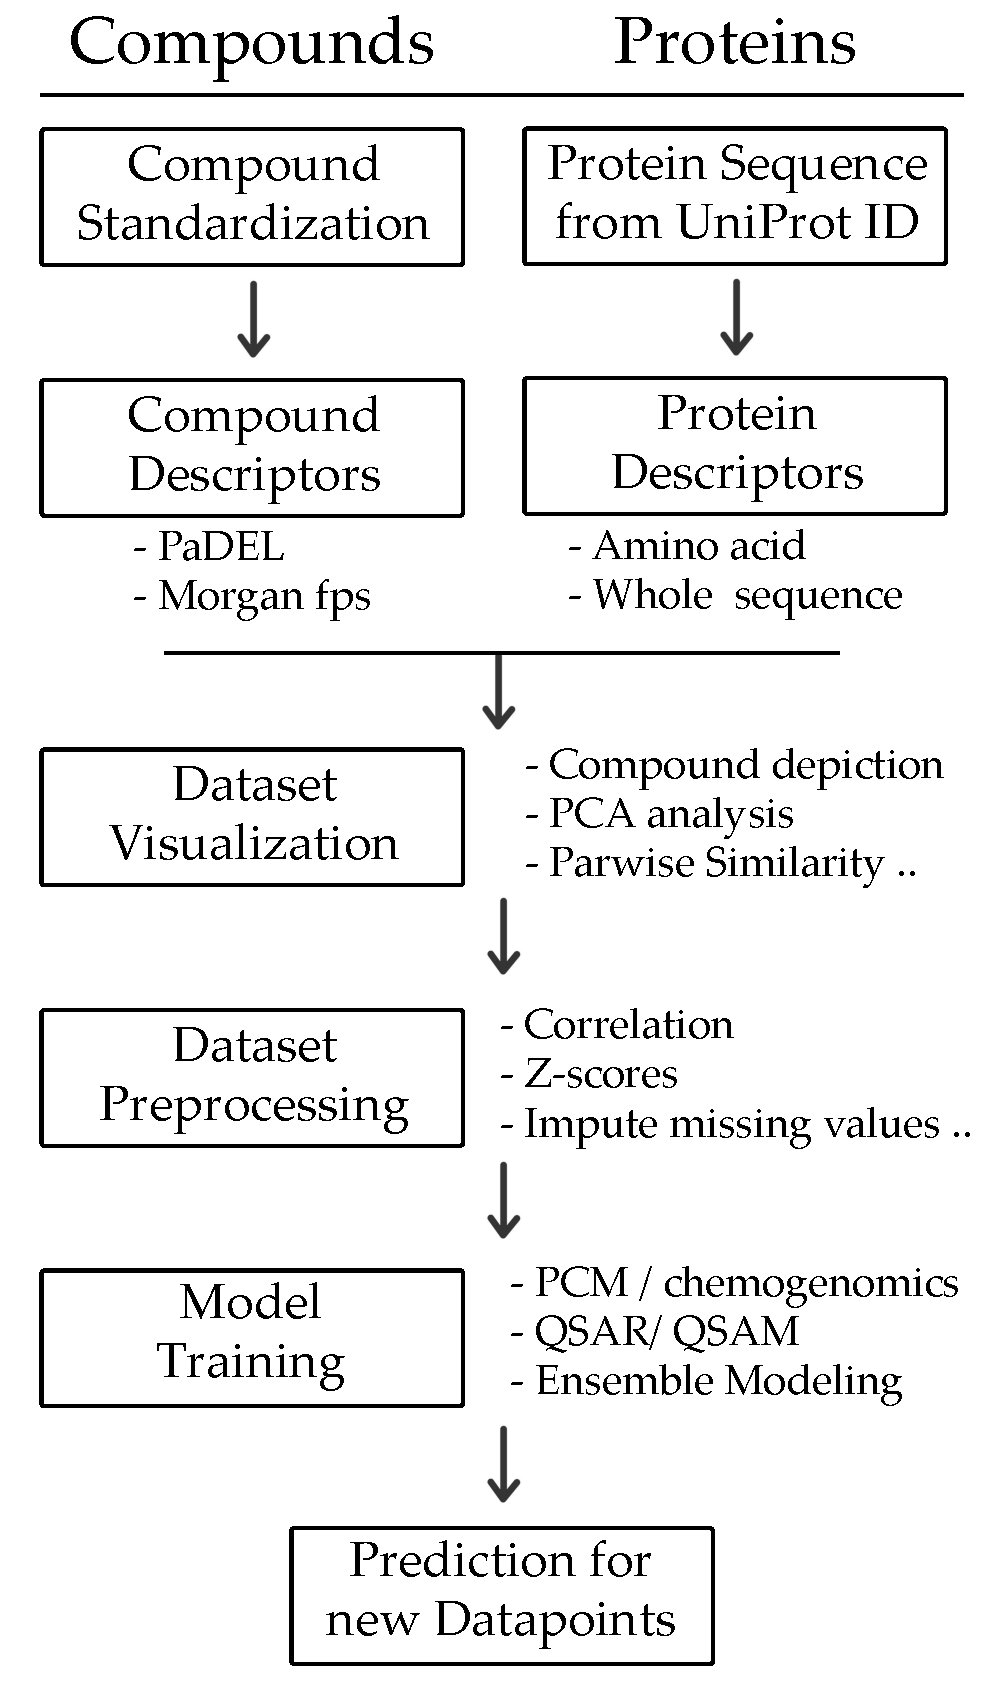
\includegraphics[width=\textwidth]{camb_outline.pdf}
%\end{center}
%\caption{}
%\label{scheme}
%\end{figure}
